\documentclass[10pt,leqno]{amsart}
\usepackage{graphicx}
\baselineskip=16pt
\usepackage{indentfirst,csquotes}

\topmargin= .5cm
\textheight= 20cm
\textwidth= 32cc
\baselineskip=16pt

\evensidemargin= .9cm
\oddsidemargin= .9cm

\usepackage{datetime}
\usepackage{wrapfig}
\usepackage{enumerate}
\usepackage{graphicx}
\usepackage{caption}
\usepackage{siunitx}
\usepackage{subcaption}
\usepackage{amsmath}
\usepackage{array,tabularx}
\usepackage{chngcntr}
\usepackage{afterpage}
\usepackage{ulem}
\usepackage{hyperref}
\usepackage{dirtytalk}
\usepackage{algorithm2e}
\usepackage{enumitem,amssymb}
\usepackage{pifont}
\usepackage{amsmath}
\usepackage{listings}
\usepackage{xcolor}
\usepackage{formal-grammar}
\usepackage{varwidth}
\usepackage{fmtcount}
\usepackage{tikz}
\usepackage{array}
\usepackage[framemethod=tikz]{mdframed} % Allows defining custom boxed/framed environments
\usepackage{cleveref}
\usepackage{microtype}
\usepackage{dirtytalk}

\usetikzlibrary{trees}
\usetikzlibrary{fit}
\usetikzlibrary{shapes}
\usetikzlibrary{arrows.meta, positioning, shadows}
\usetikzlibrary{chains,shapes.multipart}
\usetikzlibrary{external}
\usetikzlibrary{matrix}

\tikzstyle{rect} = [rectangle,fill=white, text centered]
\tikzstyle{database} = [draw, cylinder, shape border rotate = 90, aspect = 0.2]
\tikzstyle{thick-arrow} = [->, thick]
\tikzstyle{arrow} = [thick,->,>=stealth]
\tikzstyle{arrow-small} = [->,>=stealth]
\tikzstyle{simple-rect} = [rectangle, text centered, draw = black, inner sep=4mm]

\tikzset{
    doc/.style={draw, minimum height=4em, minimum width=3em, 
                fill=white, 
                double copy shadow={shadow xshift=4pt, 
                             shadow yshift=4pt, fill=white, draw}}
}

\tikzset{
    dcs/.style = {double copy shadow},
}


\newtheorem{theorem}{Theorem}[]
\newtheorem{definition}[theorem]{Definition}
\newtheorem{example}[theorem]{Example}
\newtheorem{lemma}[theorem]{Lemma}
\newtheorem{proposition}[theorem]{Proposition}
\newtheorem{corollary}[theorem]{Corollary}
\newtheorem{conjecture}[theorem]{Conjecture}

\hypersetup{
    colorlinks=true,
    filecolor=magenta,      
    urlcolor=blue,
}

\hypersetup{linkcolor=black}

\newcommand{\src}[1]{\texttt{#1}}

\lstset{basicstyle=\footnotesize\ttfamily,breaklines=true, captionpos=b}


\mdfdefinestyle{commandline}{
	leftmargin=10pt,
	rightmargin=10pt,
	innerleftmargin=15pt,
	middlelinecolor=black!50!white,
	middlelinewidth=2pt,
	frametitlerule=false,
	backgroundcolor=black!5!white,
	frametitle={LLM Output},
	frametitlefont={\normalfont\sffamily\color{white}\hspace{-1em}},
	frametitlebackgroundcolor=black!50!white,
	nobreak,
	singleextra={%
    }
}

% Define a custom environment for command-line snapshots
\newenvironment{commandline}{
	\medskip
	\begin{mdframed}[style=commandline]
}{
	\end{mdframed}
	\medskip
}

\mdfdefinestyle{warning}{
	topline=false, bottomline=false,
	leftline=false, rightline=false,
	nobreak,
	singleextra={%
		\draw(P-|O)++(-0.5em,0)node(tmp1){};
		\draw(P-|O)++(0.5em,0)node(tmp2){};
		\fill[black,rotate around={45:(P-|O)}](tmp1)rectangle(tmp2);
		\node at(P-|O){\color{white}\scriptsize\bf ?};
		\draw[very thick](P-|O)++(0,-1em)--(O);%--(O-|P);
	}
}

% Define a custom environment for warning text
\newenvironment{prompt}[1][Prompt:]{ % Set the default warning to "Warning:"
	\medskip
	\begin{mdframed}[style=warning]
		\noindent{\textbf{#1}}
}{
	\end{mdframed}
}



\title{Automatic Disease Diagnosis Using Large Language Models and Answer Set Programming}
\author{
	Ioanna Gemou
	\and
	Evangelos Lamprou
}

\begin{document}

\maketitle
\begin{abstract}
The development of automatic disease prediction systems is critically important for improving human health and supporting physicians in accurate diagnosis and treatment. Accurate diagnosis is essential for timely intervention and effective therapy, and it can also help prevent further complications and burdensome medical procedures.
Symbolic artificial intelligence has previously been applied in the medical domain \cite{Alviano_2020}. However, its adoption has been limited due to the complex knowledge bases required for such systems to operate.

The proposed method, which combines Large Language Models (LLMs) with Answer Set Programming (ASP), offers a powerful approach by providing a reliable and efficient means of generating a knowledge base that can then be used for disease prediction.
The novelty of our method lies in the combination of these two paradigms. LLMs are capable of encoding medical literature into ASP code with remarkable accuracy and deep comprehension, while ASP contributes structured reasoning and explainability. This combination enables the development of a robust disease prediction system that integrates the \textbf{accuracy and intelligence of language models} with the \textbf{explainability and efficiency of Answer Set Programming}.
Our method demonstrates promising results on the patient dataset to which it was applied.
\end{abstract}

\section{Literature Review}

\subsection{Large Language Models}

Large language models \cite{zhao2023survey} are advanced computational models designed to understand and generate human language. These models, developed using sophisticated machine learning techniques, have the ability to process and generate text in a way that closely resembles human language patterns.

Large language models, such as the \textit{GPT-4} architecture \cite{openai2023gpt4}, are trained on vast amounts of text data, allowing them to acquire knowledge across various fields and topics. These models use deep learning algorithms \cite{Sarker2021} and specifically transformer networks \cite{Dosovitskiy2020} to analyze and understand the relationships between words, phrases, and sentences. By capturing patterns and structures in the training data, these models can generate coherent and relevant responses based on given prompts.

The models are referred to as "large" because they have billions of parameters that shape their responses. The basic premise of a language model is its ability to predict the next word (referred to as a token) based on the text it has observed so far, according to the context.

Large language models possess the remarkable ability to transform text from one form to another, making them powerful tools for various language processing tasks. This characteristic underpins the idea of this work, as a significant part we deal with is the appropriate encoding of medical literature. Below we list some examples of the use of large language models \cite{Paranjape2023}:

\subsection{Difficulties in Implementing LLMs}

Large language models (LLMs) are not without errors \cite{Raj2023}, \cite{Ruis2023}. They can occasionally produce incorrect or biased responses that reflect the biases inherent in the training data. Efforts are being made to mitigate these issues through data preprocessing techniques and fine-tuning.

Overall, large language models have demonstrated tremendous potential across a wide range of applications, including natural language understanding, content creation, and human-computer interaction. Ongoing research and development in this field promise further enhancement of these models and their applications across various domains, contributing to the advancement of language processing and communication technologies.

\subsection{Answer Set Programming}

Answer Set Programming (ASP) \cite{Eiter2009} is a declarative problem-solving approach based on Logic Programming and Non-Monotonic Reasoning. The semantics of stable models and the basic language of ASP were initially formalized in the work \cite{Gelfond2000}.

Programming with this approach is done in a family of languages sometimes referred to as \textit{AnsProlog} \cite{Gelfond2002}.

The idea behind ASP is to model a problem as a set of rules and data, and then use a solver to find a solution to the problem. Solutions are represented by stable models or answer sets. The rules, data, and constraints that describe the problem are the elements of the program. Subsequently, the program is given to a solver that will find one or more solutions.

In traditional programming, transitioning from a problem to a solution requires the programmer's thorough understanding of the given problem, followed by the creation of a program that will produce the correct output when provided with an instance of the problem, which will then be interpreted as the solution.

In ASP, the transition from problem statement to a set of solutions involves the following steps \cite{Gebser2013}~(\cref{fig:asp-solving}):

\begin{figure}[htb]
    \begin{center}
\begin{tikzpicture}[node distance=4cm]
        \node [simple-rect] (problem)  at (0,0) {Problem};
        \node [simple-rect, below of=problem] (program) {Program};
        
        \node [simple-rect, right of=program] (grounder) {Grounder};
        \node [simple-rect, right of=grounder] (solver) {Solver};
        
        \node [simple-rect, right of=solver] (stable-models) {Stable Models};
        
        \node [simple-rect, above of=stable-models] (solution) {Solution};

        \draw [arrow] (problem) -- node[right] {\textbf{Modelling}} (program);
        \draw [arrow] (stable-models) -- node[left] {Interpreting} (solution);

        \draw [arrow-small] (program) -- node[above] {} (grounder);
        \draw [arrow-small] (grounder) -- node[above] {\footnotesize Grounding} (solver);
        \draw [arrow-small] (solver) -- node[above] {} (stable-models);

        \node[draw, dotted, fit=(grounder) (solver), inner sep=4mm, label=above:{Solving}] {};
\end{tikzpicture}
    \end{center}
		\caption{Solving a problem using ASP.}
    \label{fig:asp-solving}
\end{figure}

\begin{itemize}
    \item \textbf{Modeling}: The problem is modeled using ASP (Answer Set Programming) language.
    \item \textbf{Grounding}: A grounder (e.g., gringo) converts the program into a set of basic rules and facts.
    \item \textbf{Solving}: A solver (e.g., clasp) finds a solution to the problem by computing the set of stable models (answer sets).
\end{itemize}

Several solvers for ASP have been developed, such as DLV \cite{Xia2020}. In this work, we will apply the ASP system clingo \cite{Gebser2014}, which combines the grounder gringo with the clasp solver \cite{Holldobler2014} into a single application, also providing a powerful Python API for integrating the solver into other applications.

\subsection{Use of ASP in Disease Diagnosis}
Answer Set Programming (ASP) offers a powerful method for representing medical knowledge in a declarative and logical manner. Below are some common ASP methods used in the representation of medical knowledge \cite{Vinarti2019}:

\begin{itemize}
    \item \textbf{Rule-Based Representation}: ASP allows for the representation of medical knowledge as rules in the form of logical statements. These rules define relationships between medical entities such as symptoms, diseases, treatments, and patient data. For example, a rule could state that if a patient exhibits specific symptoms, it indicates the presence or absence of certain diseases.
    \item \textbf{Knowledge Base Construction}: ASP provides a framework for constructing a knowledge base that captures medical knowledge. The knowledge base consists of facts, rules, and constraints that define the information and limitations related to medical diagnosis and treatment. It may include information about disease-symptom relationships, diagnostic criteria, treatment guidelines, and patient data.
\end{itemize}

In the work \cite{Erdem2011}, new methods were introduced for effectively handling complex queries within the context of biomedical ontologies and databases, with an emphasis on extracting relevant information from these knowledge resources. These methods were applied to address demanding queries in the field of drug discovery, using biological databases in conjunction with concise explanations for complex queries related to drug discovery processes.

\section{Methodology}

\subsection{Architecture}

\begin{figure}[!h]
\begin{center}
\begin{tikzpicture}[node distance = 5cm, minimum width=2cm, minimum height=1cm]
    \node [doc, label=above:{}] (med-bib) {Medical Bibliography};
    \node [rect, draw, right=3cm of med-bib, fill=blue!50] (llm) {Large Language Model};
    \node [rect, draw, above= 1cm of med-bib, fill=orange!50] (prompt) {Prompt};
    \node [database, below left= 3cm of med-bib, fill=green!30] (knowledge-base) {Knowledge Base};
    \node [rect, draw, right of=knowledge-base] (solver) {ASP Solver};
    \node [rect, draw, below=1cm of solver] (patient) {\textit{Patient Data}};
    \node [rect, right of=solver] (diagnosis) {\textbf{Diagnosis}};

    \draw[thick-arrow] (med-bib) edge [] node [above] {} (llm);
    \draw[thick-arrow] (prompt) edge [in=90, out=0, looseness=1] node [above, sloped] {\textit{\say{please convert the following into ASP code...}}} (llm);
    \draw[thick-arrow] (llm) edge [in=90, out=270, looseness=1] node [below] {ASP Program} (knowledge-base);
    \draw[thick-arrow] (knowledge-base) edge [] node [above] {} (solver);
    \draw[thick-arrow] (solver) edge [] node [above] {} (diagnosis);
    \draw[thick-arrow] (patient) edge [in=270, out=180, looseness=1] node [above] {} (knowledge-base);

\end{tikzpicture}
\end{center}
\caption{The diagnostic process using the proposed method. Medical literature,
	through the use of a large language model, is transformed into an ASP
	program. Subsequently, this program is executed by an ASP solver, which
	produces the final diagnosis based on the data of each patient.}
    \label{fig:architecture}
\end{figure}

Our goal is to extract a knowledge base from unstructured text \cite{ré2014feature}. Our architecture (Figure \ref{fig:architecture}) includes the following stages:

\begin{itemize}
	\item Collecting medical literature related to the diseases/conditions under examination.
	\item Creating an appropriate prompt for converting medical literature into ASP code.
	\item Adding the ASP code generated by the large language model to the knowledge base.
	\item Adding relevant patient data (symptoms, medical examination results) to the knowledge base.
	\item Producing the final diagnosis (or set of possible diagnoses) as answer set(s), after the solver reasons over the final knowledge base.
\end{itemize}

\subsection{Prompt Construction}

Despite their high capabilities in executing instructions, large language
models still have low reliability \cite{bowman2023things}. Thus, a relatively
new programming methodology known as prompt engineering has emerged
\cite{liu2021pretrain, promptingguidePromptEngineering}. In order to convert
medical literature into code suitable for execution in an ASP solver, we had to
construct quality prompts so that the generated code is in the desired form
(Figure \ref{fig:bad-prompt}, Figure \ref{fig:good-prompt}).

\begin{figure}[!h]
\centering
\begin{prompt}
\textit{Medical Text...}

The above paragraph refers some common symptoms of pneumonia.
Give me a Clingo script so that based on symptoms I can diagnose pneumonia.
\end{prompt}


\begin{commandline}
\begin{verbatim}

symptom(cough).
symptom(cough_with_mucus).
symptom(chest_pain).
symptom(headache).
...

diagnosis(pneumonia) :- symptom(cough), 
                        symptom(chest_pain), 
                        symptom(headache), 
                        symptom(arthralgia),
                        ...
\end{verbatim}
\end{commandline}

\caption{A simple prompt that does not yield satisfactory results.}
\label{fig:bad-prompt}
\end{figure}

\begin{figure}[!h]
\begin{prompt}
\textit{Medical Text...}

The above paragraph refers some common symptoms of pneumonia.
Give me a Clingo script so that based on symptoms I can diagnose pneumonia.

In the clingo script that you produced before, make some changes in diagnosis rule like:
\src{diagnosis(pneumonia) :- has(symptom(x)), has(symptom(y)) ...}

Include some alternative diagnosis for pneumonia.
Create rules based on one symptom being linked to another.
\end{prompt}


\begin{commandline}
\scriptsize
\begin{verbatim}
symptom(cough).
symptom(cough_with_mucus).
...


linked_symptom(cough_with_mucus, wheezing).
linked_symptom(cough_with_mucus, shortness_of_breath).

...

has(symptom(Symptom2)) :- has(symptom(Symptom1)), 
              linked_symptom(Symptom1, Symptom2).


diagnosis(pneumonia) :- has(symptom(cough)),
                        has(symptom(cough_with_mucus)),
...

diagnosis(pneumonia) :- has(symptom(cough_with_mucus)),
                        has(symptom(chest_pain)),
...
\end{verbatim}
\end{commandline}
\caption{A good prompt that yields satisfactory results.}
\label{fig:good-prompt}
\end{figure}

\subsection{Construction of a Logical Program}

The knowledge base initially consists of a set of symptoms and medical indicators in the form:

\begin{align}
    symptom(s). & \; s \in \{ \text{cough, chest pain, rash}, \dots \} \\
    indicator(i). & \; i \in \{ \text{low MCV, high TIBC}, \dots \}
\end{align}

We represent a patient who has a certain symptom or tested positive for a certain test as:

\begin{equation}
    has(x). \; x \in S \cup I
\end{equation}

The logical propositions based on which our system will draw conclusions are in the form:

\begin{align}
    diagnosis(d_1) & \longleftarrow has(x_1) \land has(x_2) \land \dots \\
    diagnosis(d_1) & \longleftarrow has(x_1) \land has(x_3) \land \dots \\
    diagnosis(d_2) & \longleftarrow has(x_3) \land has(x_4) \land \dots
\end{align}

We also take into account the correlation between certain symptoms. For example, there has been a noted connection between skin diseases and headaches in certain patients\cite{migraine-hives}. Sometimes, symptoms may lead to the development of other symptoms. Such relationships are encoded in our knowledge base through a rule of the form:

\begin{align}
    has(symptom(S2)) \longleftarrow has(symptom(S1)) \land linked\_symptom(S1, S2).
\end{align}

The corresponding data will be as follows:

\begin{align}
    linked\_symptom(grunting, chest\_retractions).\\
    linked\_symptom(nasal\_flaring, chest\_retractions).
\end{align}

However, it is expected that a patient will not exhibit \textit{all} recorded symptoms. We want to provide a controllable way for our system to make alternative predictions in cases where the medical staff does not have all the information about the patient's condition. Thus, we add the following choice rule, which adds a set of possible symptoms for the patient to the knowledge base.

\begin{equation}
    \{ add(symptom(S)) : symptom(S) \}.
\end{equation}

Additionally, we require the solver to find at least one diagnosis.

\begin{equation}
    \bot \longleftarrow \sim diagnosis(\_)
\end{equation}

Finally, we minimize the number of "false" diagnoses so that the solver arrives at a diagnosis with as few assumptions as possible.

\begin{equation}
    \#minimize \{ 1, S : add(S) \}
\end{equation}

This way, our system guarantees that it will produce at least one prediction, which will be based as much as possible on valid information available about the patient.

\subsection{Explainability of Diagnoses}

Symbolic artificial intelligence has a major advantage over subsymbolic approaches due to its explainability. The relationships between the facts and conclusions that a system, which executes a symbolic mechanism, reaches are clearly defined. However, ASP solvers like \textit{Clingo} do not provide\footnote{At the time of writing this paper.} intuitive traces of their reasoning processes. There has been research on linking logical propositions with their justifications \cite{cabalar2014causal}. Consider the following logic program; the connection of the logical propositions with their causes is presented in the form of a graph in Figure \ref{fig:causal-g}. This structure allows us to explain the conclusions of a symbolic logic solver.

\begin{equation}
\begin{aligned}[b]
    l :& punish \longleftarrow drive, drunk \\
    m :& punish \longleftarrow resist \\
    e :& prison \longleftarrow punish \\
    d :& drive \\
    k :& drunk \\
    r :& resist \\
\end{aligned}
\label{eq:example-cg}
\end{equation}

\begin{figure}
    \centering
    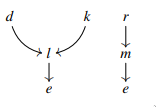
\includegraphics{assets/causal_g.png}
    \caption{Causal graph of logic program (eq. \ref{eq:example-cg}).}
    \label{fig:causal-g}
\end{figure}

The tool \textit{xclingo}\footnote{\url{https://github.com/bramucas/xclingo2}} \cite{Cabalar_2020} allows the presentation of justifications regarding the results given by the solver \textit{Clingo}. This is achieved by adding a \src{trace} corresponding to the rules of our logic program. Providing a clear explanation of how the system reached specific conclusions can help identify potential errors in the creation of the knowledge base and provide the system user with a rationale for the final outcome. This is particularly important when the application is used in medical contexts.

\section{Results}

To evaluate our system, we used publicly available patient data\footnote{\url{https://www.kaggle.com/datasets/itachi9604/disease-symptom-description-dataset?select=dataset.csv}}. The symptoms of each patient were fed into the system as input. Our knowledge base consists of the combination of all rules derived from encoding the medical literature. A successful prediction is defined when the actual disease of the patient matches the final prediction of the ASP solver.

\begin{table}[h]
    \centering
    \begin{tabular}{lcc}
    \hline
    Diseases & Size of Knowledge Base & Accuracy \\
    \hline
    \hline
    Chicken Pox      &  66  & 95\% \\
    Pneumonia        &  75  & 100\% \\
    Common Cold    &   44 & 100\% \\
    \hline
    \end{tabular}
    \caption{Accuracy of the method for some indicative diseases.}
\end{table}

The accuracy of our model can reach very high rates but requires the input of a large number of rules into the knowledge base. We define the size of the knowledge base as the number of logical terms within the ASP program corresponding to each of the diseases.

In the program we developed, we also added the capability to explain the diagnosis, where we utilize the \src{xclingo} tool to create a graph that depicts the associations followed by our system for its predictions.

\begin{lstlisting}[caption={Part of the explanation for the diagnosis of the
disease chickenpox. The decision tree diagram shows the associations between
different symptoms and how our system arrives at its conclusions.},
label=lst:terms]{Name}
  *
  |__diagnosis(chickenpox)
  |  |__has(symptom(itching));has(symptom(itching))
  |  |__has(symptom(fatigue));has(symptom(fatigue));has(symptom(fatigue));has(symptom(fatigue));has(symptom(fatigue))
  |  |__has(symptom(lethargy))
  |  |  |__has(symptom(fatigue));has(symptom(fatigue));has(symptom(fatigue));has(symptom(fatigue));has(symptom(fatigue))
  |  |  |__linked_symptom(fatigue,lethargy)
  |  |__has(symptom(high_fever))
  |  |  |__has(symptom(mild_fever));has(symptom(mild_fever))
  |  |  |  |__has(symptom(loss_of_appetite));has(symptom(loss_of_appetite))
  |  |  |  |__linked_symptom(loss_of_appetite,mild_fever)
  |  |  |__linked_symptom(mild_fever,high_fever)
  |  |__has(symptom(loss_of_appetite));has(symptom(loss_of_appetite))
  |  |__has(symptom(mild_fever));has(symptom(mild_fever))
  |  |  |__has(symptom(loss_of_appetite));has(symptom(loss_of_appetite))
  |  |  |__linked_symptom(loss_of_appetite,mild_fever)
  |  |__has(symptom(swelled_lymph_nodes))
  |  |  
  ...
\end{lstlisting}

\section{Conclusions}

In this paper, a methodology for the automatic prediction of diseases was
presented, which includes the encoding of medical literature and its
transformation into ASP code through a large language model. The operation of
large language models and ASP was presented, with specific reference to the
role each technology plays in the final system. We also showed our architecture
and how these technologies will be combined, while providing specific
implementation details that we developed for both the creation of quality
prompts for the large language model and the structure of the rules in the
final ASP knowledge base. Finally, we executed predictions on certain diseases
for which we created the knowledge base using our methodology and presented the
results. Our method appears to have promising outcomes and offers reliable
high-accuracy predictions along with their explanations.

Future work includes extending the method to cover more diseases.
Simultaneously, it would be useful to create a graphical interface through
which someone could input patient data and receive possible diagnoses.
\newpage
\bibliographystyle{unsrt}
\bibliography{bib}

\end{document}
